\newpage
\section{Implementation}
\label{sec:used GAN discussion}
% dire che adesso andrò a descrivere le reti che ho usato per ottenre una rete in grado di generare immagini quando condizioanta a uno sketch. 
In this chapter are described the generative adversarial networks used to generate synthetic images starting from a sketch.
% *******************************************
\subsection{StyleGAN}
\label{section:StyleGAN}
StyleGAN \cite{StyleGAN} is a state-of-the-art deep learning generative model developed by NVIDIA in 2018 for producing realistic-looking images. The model is based on Generative Adversarial Network (GAN) architecture, in particular, is built upon the foundation of the ProGAN. It takes inspiration from the concept of “style transfer” introduced in \cite{ImageStyleTransfer}  to generate unique images. This involves using neural representations to separate and recombine the content and style of images. \\
It is designed to generate high-resolution images of faces, but can also be adapted to generate other types of images as well. The key feature of StyleGAN is its ability to generate high-resolution images while also controlling various aspects of the image style, such as colour, texture, and overall composition. \\ \\
The main idea behind StyleGAN is to use a deep neural network that is trained to generate images from a random noise input. This noise input is then transformed into a feature representation, which is fed into a generator network. The generator network uses a series of convolutional layers to upsample the feature representation and generate the final image. The generator in StyleGAN begins by using a learned constant input and then modifies the style of the image in every convolution layer based on the latent code. This direct control allows for the adjustment of the strength of the image's features at various scales. The inclusion of noise directly injected into the network results in the automatic, unsupervised separation of high-level attributes such as pose and identity from stochastic variations like freckles and hair in the generated images. This design makes it possible to perform intuitive mixing and interpolation operations that are specific to different scales.
\\ \\
The design of StyleGAN is different from the one of the traditional GANs, since the latent code is not provided to the generator through an input layer. However, the generator starts by using a $4\times4\times512$ constant to start the image synthesis process, and uses a non-linear mapping network to map the input latent code $z$ to an intermediate space. The non-linear mapping function is a function $f:Z\rightarrow W$ where $Z$ is the input latent space and $W$ is the intermediate latent space. This mapping network outputs a vector that controls the style of the generated image by integrating it into the generator model through the adaptive instance normalisation layer. This vector provides the ability to dictate the style of the synthetic image.
For simplicity, the authors set the dimensionality of both the input latent space and the intermediate latent space to $512$ and the mapping is done using a $8$-layer Multi-layer Perceptron (MLP). This choice of dimensionality is arbitrary and could potentially be changed in other implementations.\\
The purpose of the Mapping Network is to convert an input vector into an intermediate vector that governs different visual attributes. This is challenging as the input vector must adhere to the probability density of the training data, therefore it conducts to an entanglement of features. To solve this issue, the Mapping Network is used to create an intermediate vector that does not have to follow the distribution of the training data, allowing for a disentangled representation. Given the inapplicability of previous methods for determining disentanglement in the latent space in this case, the authors introduced two new automated metrics: perceptual path length and linear separability. These metrics enable them to quantify the disentanglement of the generator. Their results show that compared to a conventional generator architecture, their generator allows for a more linear and less entangled representation of various factors of variation.\\ \\
\begin{figure}[htbp]
\centering
  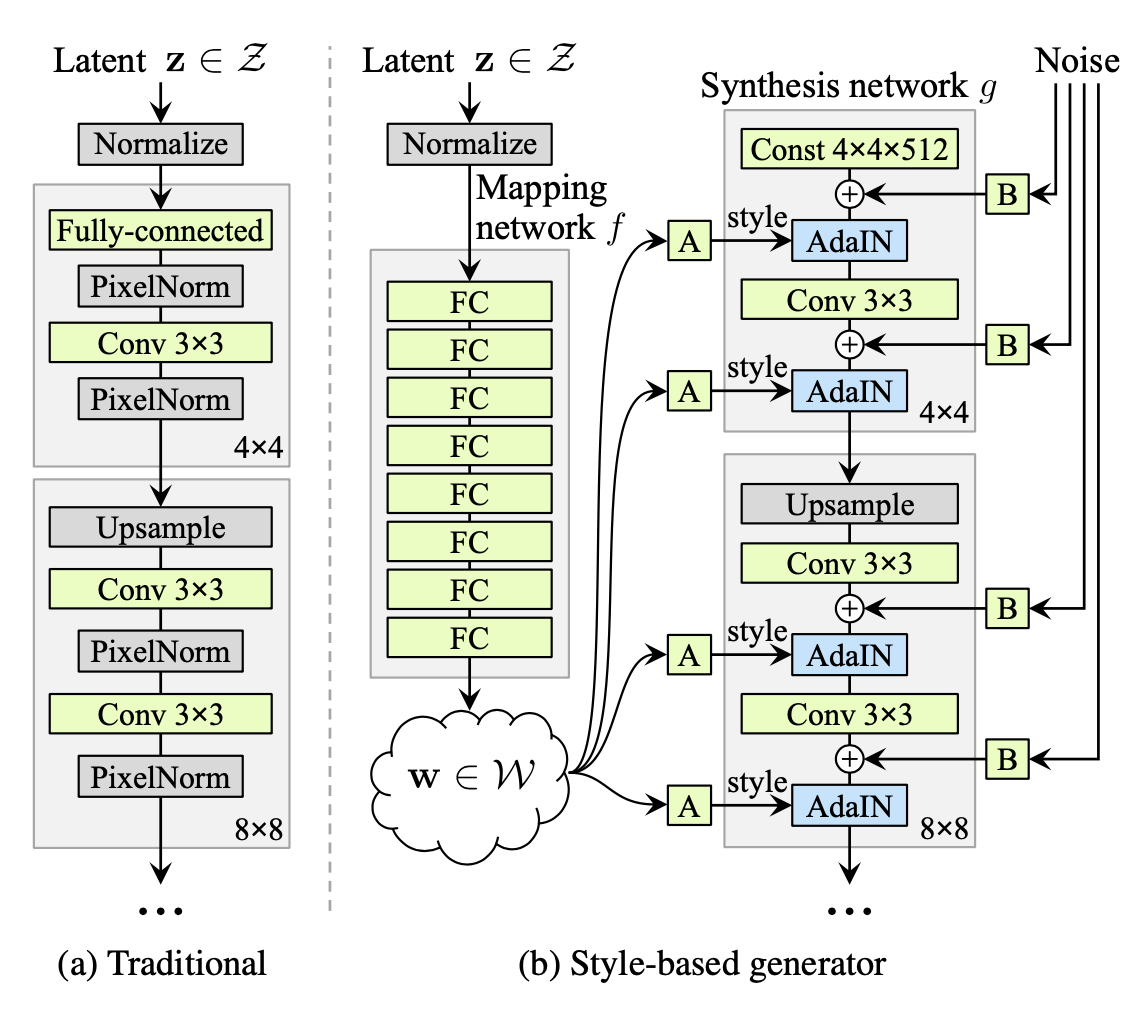
\includegraphics[scale=0.5]{figures/styleGAN-generator.png}
  \caption{(a) traditional GAN architecture, (b) Style GAN architecture. Image taken from \cite{StyleGAN}. The mapping network consists of 8 layers, while the synthesis network g consists of 18 layers (two for each resolution starting from $4^2$). The “A” block stands for the affine transform, and the “B” is the block that applies per-channel scaling factor to the input Gaussian noise.}
  \label{fig:StyleGAN architecture}
\end{figure}
The output of the Mapping Network is 512×1, the same size as the input layer. The StyleGAN generator model is now referred to as the “synthesis network” due to the integration of the new mapping network into its architecture, its architecture can be seen in fig. \ref{fig:StyleGAN architecture}(b), while fig. \ref{fig:StyleGAN architecture}(a) shows a traditional GAN architecture.
%
The AdaIN layer \cite{ArbitraryStyleTransfer} is an extension of the Instance Normalization layer which can adapt to different styles instead of being able to normalise to a single, specified style. The AdaIN layer integrates information from a learned encoding of the style of the image into the generator network to allow for control over the style of the generated image. This layer is added at each resolution level of the synthesis network to provide a unique visual expression of features at each level. The AdaIN layer integrates information from a learned encoding of the style of the image into the generator network to allow for control over the style of the generated image.
The AdaIN modules shift and scale the output through the layers in the synthesis network, promoting the significance of relevant filters in each convolutional layer. This helps the generator differentiate between important and insignificant features. It can be considered as an internal feedback mechanism, where the mapping network learns to encode the $W$ vector by focusing on the most relevant features. 
The AdaIN operation starts by normalising each channel to have zero mean and unit variance, before using the provided style information to apply scales and biases to each channel. The scale and bias values adjust the relative importance of each feature in the subsequent convolution operation. However, the original statistics of the input are not taken into account because of the normalisation step. As a result, each AdaIN operation only controls one convolution before being overridden by the next AdaIN operation.
The AdaIN operation receives a feature map $x_i$ and a style input $y=(y_s,y_b)$, and it is defined as:
\begin{equation}
    \mbox{AdaIN}(x_i,y)=y_{s,i}\frac{x_i - \mu (x_i)}{\sigma(x_i)}+y_{b,i}
\end{equation}

\noindent where $\mu(x_i)$ is the mean, $\sigma(x_i)$ is the variance, while for scaling and shifting $y_{s,i}$ and $y_{b,i}$ are used respectively. Since $y$ consists in a scaling and shifting factors, its dimensionality is twice the number of feature maps on that layer.
This process helps to preserve the content information from the content input while allowing the style information from the style input to be applied to the output.
Additionally, each layer of the synthesis network is fed with uncorrelated Gaussian noise before the AdaIN operation in order to generate stochastic details. Incorporating random noise at each style block enables more precise control over the model's generated details, including finer features like freckles, beard, wrinkles, and dimples. Without this noise, these small details would be overpowered by larger, more prominent features. It is evident that the noise only impacts the stochastic elements, preserving the overall composition and high-level features such as identity.\\
The mixing regularisation technique is used to promote even more the localisation of styles in the generator. During training, a portion of the images is generated using two random latent codes instead of just one. This process, called style mixing, involves switching from one latent code to another at a randomly chosen point in the synthesis network. The mapping network processes the latent codes, $z_1$ and $z_2$, producing the corresponding styles $w_1$, $w_2$, which control the styles applied before and after the crossover point, respectively. This regularisation method prevents the network from assuming a correlation between adjacent styles. \\
%%
%%%%%%%%%%%%%%% -.----------------
\noindent The authors showed experimentally that the redesign of the generator not only preserves image quality but, in fact, significantly enhances it. To demonstrate this, they computed the Fréchet inception distances (FID) for various generator architectures on a few available datasets.
The authors' results suggest that a style-based design is superior to the conventional GAN generator architecture in all aspects. This superiority is demonstrated through established quality metrics, and our findings on the separation of high-level features and stochastic effects, as well as the linearity of the intermediate latent space, all point towards a deeper understanding and control of GAN synthesis.
Furthermore, their average path length metric can be easily used as a regularisation term during training, and a similar approach could be applied to the linear separability metric.

\subsection{StyleGAN2}
\label{section:StyleGAN2}
StyleGAN2 (2020) is an improvement of (\ref{section:StyleGAN}) for synthesizing high-resolution images developed by NVIDIA. This new version is based on the previous one, but with some differences \cite{Karras2019stylegan2}.
The authors of StyleGAN2 discovered that styles were not only capable of capturing and transferring the essence of an image, but also transferring visual distortions such as water droplets or smudges.
They linked these visual distortions to the AdaIN layers, and therefore they made some changes to them in order to eliminate the artifacts. To overcome this issue, they came up with a new approach to the AdaIN layers, which were previously used as direct inputs to the network. Instead, they integrated the AdaIN layers within the convolutional layers, this integration allowed for parallel computation, significantly boosting the speed of training the model by up to 40\% and reducing the appearance of visual distortions. \\
The authors replace the AdaIN operator with a weight modulation and demodulation step, where the modulation adjusts each feature map of the convolution based on the style. 
%%% METTO ?? 
%This can be achieved by scaling the weights of the convolution, as showed in the following equation: 
%\begin{equation}
%    w'_{ijk} = s_i \cdot w_{ijk}
%\end{equation}
%where $w$ are the original weights, $w'$ are the modulated weights, $s_i$ is the scale corresponding to the $i$th input feature map, and $j$ and $k$ represent the convolution's output feature maps and spatial footprint, respectively.
The authors discovered that the strong location preference for facial features in StyleGAN images was due to progressive growing. To address this, they took inspiration from the “Multi-Scale Gradients for Generative Adversarial Networks” paper by Animesh Karnewar and Oliver Wang \cite{karnewar2019msg} and incorporated the idea of multiple scale gradient using a single architecture. The authors developed a new architecture that employs multiple scales of image generation, which is achieved through the utilisation of a resnet-style skip connection that links lower resolution feature maps to the final generated image.
A further difference between the two version of StyleGAN is the introduction of a normalisation term to the loss function in order to make the latent space more uniform and smoother. By doing so, the mapping of images in and out of the latent space becomes more controlled, enabling more controlled image generation. Additionally, this improved relationship between the latent space and generated images allows for images to be generated along a path in the latent space. The regularisation term added to the loss is driven by the goal to keep vector lengths consistent no matter which direction they point in, and it is formulated as:
\begin{equation}
    \mathbb{E}_{\mathbf{w,y}\sim \mathcal{N}(0,1)}=(\| \mathbf{J_w}^T\mathbf{y}\|_2 - a)^2
\end{equation}
where $\mathbf{y}$ are random images with normally distributed pixel intensities, $\mathbf{w} \sim f(\mathbf{z})$, where $\mathbf{z}$ are normally distributed. The local metric properties of the generator's mapping function $g(\mathbf{w}): \mathcal{W}\rightarrow \mathcal{Y}$ are represented by the Jacobian matrix $\mathbf{J_w}$, which is defined as $\mathbf{J_w}=\partial g(\mathbf{w})/\partial \mathbf{w}$.
The value of the constant $a$ is dynamically determined during the optimisation process through the calculation of the long-term exponential moving average of the vector lengths $\| \mathbf{J_w}^T\mathbf{y} \|_2$. This allows the optimisation to automatically find an appropriate global scale for the process.\\
This regularisation term is known as \textit{path length regularisation}, and its implementation of has proven to be highly beneficial in practice, leading to the development of more stable and consistent models. This makes the process of exploring and experimenting with different architectural designs much more manageable. Additionally, it has been noted that the smoother nature of the generator as a result of this regularisation makes it significantly easier to perform inversion.\\ \\
Additionally, they observe that there was no need to compute the regularisation term every time the loss was computed, therefore in this way they could obtain a decrease in the computational cost and also in the overall memory usage. They applied a lazy regularisation and evaluate the regularisation terms every $k$ training iterations.\\
To summarise the improvements made in the second version of StyleGAN, which leads to the removal of artifacts in generated images, enforcement of smoother latent space interpolation and reduction of the strong location preference for facial image features, are:
\begin{itemize}
    \item weight demodulation
    \item path length regularisation
    \item lazy regularisation
    \item no growing
\end{itemize}
What they achieved with this improvement are also a faster learning time and an improvement in image quality.

%%%%%%%%%%%%%%%%%%%%%%%%%%%%%%%%%%%%%%%%%%%%%%%%%%
\subsection{pSp Framework}
\label{section:pspFramework}
Pixel2Style2Pixel (pSp) is a novel image translation framework that leverages the powerful representation capabilities of a pre-trained StyleGAN2 generator and the extended $\mathcal{W}+$ latent space. The pSp framework is designed to tackle the task of transforming an input image into a target image, preserving the content of the original image while adopting the style of another.
In the paper, it is proposed a new encoder network, based on a Feature Pyramid Network, that is capable of directly encoding real images into the $\mathcal{W}+$ space. \\
The encoder that the authors built is able to directly reconstruct real input images, enabling latent space manipulations without the need for time-consuming optimisation. However, this approach is limited as the input image must be invertible, meaning that it must have a latent code that can reconstruct it. This is a critical limitation since in conditional image generation the input image do not stay in the same StyleGAN domain. The solution proposed by the authors is to utilise the encoder jointly with the pre-trained StyleGAN generator as a complete solution for image-to-image translation, thereby overcoming the limitation of the encoder's requirement. \\
The input images are transformed into the desired output latents through direct encoding, which are then processed by StyleGAN to generate the desired output images. In this way, StyleGAN can be used for image-to-image translation also in the case when the input and output images belong to different domains.\\
The straightforward way to encode an input image into the $\mathcal{W}+$ is to extend the encoder backbone with a feature pyramid in order to produce three levels of features maps of spatial resolution, which are a coarse, medium and fine.
%therefore divide the different styles inputs in three categories that are: coarse, medium and fine.
%extract a 512-dimensional vector from the last layer of the encoder network. However, this method is limited in its ability to fully capture finer details of the original image due to the bottleneck. To overcome this limitation, the authors used a discovery made by StyleGAN's authors where they found out that different levels of detail in an image can be represented by different styles inputs which are grouped into three categories: coarse, medium, and fine. Therefore, they extended the encoder backbone with a feature pyramid in order to produce three levels of feature maps.
The styles are extracted from different scales of the pyramid using an intermediate network called \textit{map2style}, and are inserted directly into the fixed, pre-trained StyleGAN2 generator in correspondence to their scale to generate the final output image.
The \textit{map2style} is a small fully convolutional network which reduces the spatial size using a set of 2-strided convolutions followed by LeakyReLU activation functions. It is trained to extract the learned style from the corresponding feature map for each of the 18 target styles. Figure \ref{fig:pSp encoder architecture} illustrates the pSp architecture.
 \begin{figure}[htbp]
\centering
  \includegraphics[scale=0.43]{figures/psp-architecture.png}
  \caption{Pixel2Style2Pixel architecture. Image taken from \cite{pSp}}
  \label{fig:pSp encoder architecture}
\end{figure}

\noindent Additionally, they wanted to design the encoder to learn the latent code based on an average style vector in order to improve the initialisation. Therefore, they defined an average style vector $\mathbf{\Bar{w}}$ of the pretrained generator, and given an input image $\mathbf{x}$ the output of their model is defined as:
\begin{equation}
    pSp(\mathbf{x}) := G(E(\mathbf{x}) + \mathbf{\Bar{w}})
\end{equation}
where $E(\cdot)$ is their encoder while $G(\cdot)$ is the StyleGAN2 generator.\\
For the loss function, the authors used a weighted combination of several functions, since they observe that this combination allowed to obtain a more accurate encoding into StyleGAN, defined as: 
\begin{equation}
    \label{eq:pSpTotalLoss}
    \mathcal{L}(\mathbf{x}) = \lambda_1 \mathcal{L}_2(\mathbf{x}) + \lambda_2 \mathcal{L}_{LPIPS}(\mathbf{x}) + \lambda_3\mathcal{L}_{reg}(\mathbf{x}) + \lambda_4\mathcal{L}_{ID}(\mathbf{x})
\end{equation}
where $\lambda_1,\lambda_2,\lambda_3,\lambda_4$ are constants used to define the loss weights, and $\mathcal{L}_2$ loss is the pixel-wise loss:
\begin{equation}
    \label{eq:l2Loss}
    \mathcal{L}_2 =  \| \mathbf{x} - pSp(\mathbf{x})  \|_2
\end{equation}
 $\mathcal{L}_{LPIPS}$ is the LPIPS loss to learn perceptual similarities, with $F(\cdot)$ denoting the perceptual feature extractor:
\begin{equation}
    \label{eq:lpips-loss}
    \mathcal{L}_{LPIPS} = \| F(\mathbf{x} - pSp(\mathbf{x}) \|_2
\end{equation}
$ \mathcal{L}_{reg}$ is the regularisation loss to guide the encoder to produce latent style vectors that are closer to the average latent vector:
\begin{equation}
    \label{eq:regularizationLoss-psp}
    \mathcal{L}_{reg} = \| E(\mathbf{x}) - \mathbf{\Bar{w}}\| _2
\end{equation}
and finally $ \mathcal{L}_{ID}$ is a loss measuring the cosine similarity between the output image and its source since they want to preserve input identity:
\begin{equation}
    \label{eq:identityLoss}
    \mathcal{L}_{ID}(\mathbf{x}) = 1 - \langle R(\mathbf{x}) - R(pSp(\mathbf{x}))\rangle
\end{equation}
where R represent the ArcFace pretrained network \cite{arcface2018}, which is a type of loss function that aims to increase the separability between classes by adding a margin to the cosine similarity between features of an image and the weight vector of the classifier.
%The authors tested the pSp architecture on two kind of conditional image generation: generating face-images starting from sketches and generating images from mantic segmentation maps. They show that, with minor modifications, their encoder can effectively leverage the power of StyleGAN to produce high-quality and diverse outputs. The training process for these two tasks is similar to that of the encoder, where the input is the conditioned image and the target is the corresponding real image. During inference, multiple images can be generated by performing style-mixing on the fine-level features. The process involves taking layers 1 to 7 from the latent code of the input image and layers 8 to 18 from a randomly drawn w vector.


%%%%%%%%%%%%%%%%%%%%%%%%%%%%%%%%%%%%%%%%%%%%%%%%%%%


\subsection{Restyle}
\label{section:restyle}
In the area of unconditional image synthesis, Generative Adversarial Networks have recently achieved outstanding results. 
It is essential for trained GANs to be able to invert an image into its matching latent code, since doing so allows them to manipulate real-world images while exploiting the network's rich semantics.
One such model is StyleGAN, which is capable of synthesizing highly realistic images, as discussed in \ref{section:StyleGAN}. However, there is a major drawback to StyleGAN: it only allows for the synthesis of new images in a specific style, meaning that it cannot change the style of an existing image.

\noindent This limitation has motivated the development of the ReStyle algorithm \cite{alaluf2021restyle}, which is a residual-based StyleGAN encoder that can change the style of an existing image. The ReStyle algorithm is based on the iterative refinement of a residual encoding that transforms the input image into a feature representation compatible with the StyleGAN generator. In this way, ReStyle allows for style transfer from a pre-trained StyleGAN2 model to a given input image.\\
In the paper, the authors presented a new encoder-based inversion approach for accurate image inversion. They observed that achieving precise inversion in a single attempt was challenging, so they introduced a novel method, called \textit{ReStyle}, that employs an iterative process to carry out the inversion. This method uses a feedback mechanism to repeatedly feed the output of each iteration back into the encoder together with the original input image. This enables the encoder to use the knowledge gained from previous iterations to focus on the important parts necessary to reconstruct the input image with a certain level of accuracy.\\
Their objective was to train an encoder $E$ capable of inverting real-world images into the extended $\mathcal{W}+$ latent space of a previously trained StyleGAN generator $G$. Where the goal must be achieved through multiple steps $N>1$, with each step consisting of a single forward pass through both the encoder and the StyleGAN generator. From a mathematical point of view, they wanted to generate an image $\hat{\textbf{y}} = G(E(\textbf{x}))$, where $\textbf{x}$ is a given input image, in such a way that $\hat{\textbf{y}} \approx \textbf{x}$. To reach this goal, the encoder was trained while the StyleGAN generator remained fixed, since it is pre-trained.
%
\subsubsection{ReStyle training}
For training the encoder network to perform the inversion task, a set of losses are introduced. The losses used, which are also used by most encoder-based methods, are a L2 loss, which measures the difference between the reconstructed image and the original image pixel-wise, and a perceptual loss, such as LPIPS, which measures the difference between the two images in terms of their high-level features. The training process of the encoder is guided by the losses, which are computed at each forward step. The encoder weights are then updated according to the computed losses via back-propagation. As stated above, ReStyle works by concatenating the input image $\textbf{x}$ with the current prediction of the reconstructed image $\hat{\textbf{y}}$, resulting in an extended 6-channel input $\textbf{x}_t$:
\begin{equation}
\label{eq:concatenationXandCurrentPred}
    \textbf{x}_t := \textbf{x} \| \hat{\textbf{y}}_t
\end{equation}
At this point the encoder E has to compute the residual code based on the latent code just predicted, and then it updates the new prediction for the latent code, as shown in equations \ref{eq:residualComputation} and \ref{eq:latentCodeUpdate}, respectively.
%update the latent code's prediction to the inversion of the input image, as shown in equations \ref{eq:residualComputation} and \ref{eq:latentCodeUpdate}, respectively.
\begin{equation}
    \label{eq:residualComputation}
    \Delta_t := E(\textbf{x}_t)
\end{equation}
\begin{equation}
    \label{eq:latentCodeUpdate}
    \textbf{w}_{t+1} \xleftarrow{} \Delta_t + \textbf{w}_t
\end{equation}
The updated prediction of the reconstructed image is obtained by passing the latent code $\textbf{w}_{t+1}$ to the generator, as defined in equation \ref{eq:updatePredictionOfReconstructed}. Finally, the updated estimate $\hat{y}_{t+1}$ is used in the following step, as specified by equation \ref{eq:concatenationXandCurrentPred}.
\begin{equation}
    \label{eq:updatePredictionOfReconstructed}
    \hat{\textbf{y}}_{t+1} := G(\textbf{w}_{t+1})
\end{equation}

\subsubsection{ReStyle Encoder architecture}
 The ReStyle encoder (fig. \ref{fig:ReStyle encoder architecture}) is design as a variation of the architecture described in \ref{section:pspFramework} and in \cite{e4e}. Instead of obtaining the style features from three intermediate levels in the encoder, all style vectors are derived from the final 16×16 feature map. To do so, k different \textit{map2style} blocks are employed to reduce the size of the feature map and produce the corresponding 512-dimensional style input, where $k$ is the number of style inputs in the StyleGAN generator, as introduced in \ref{section:pspFramework}.
 \begin{figure}[htbp]
\centering
  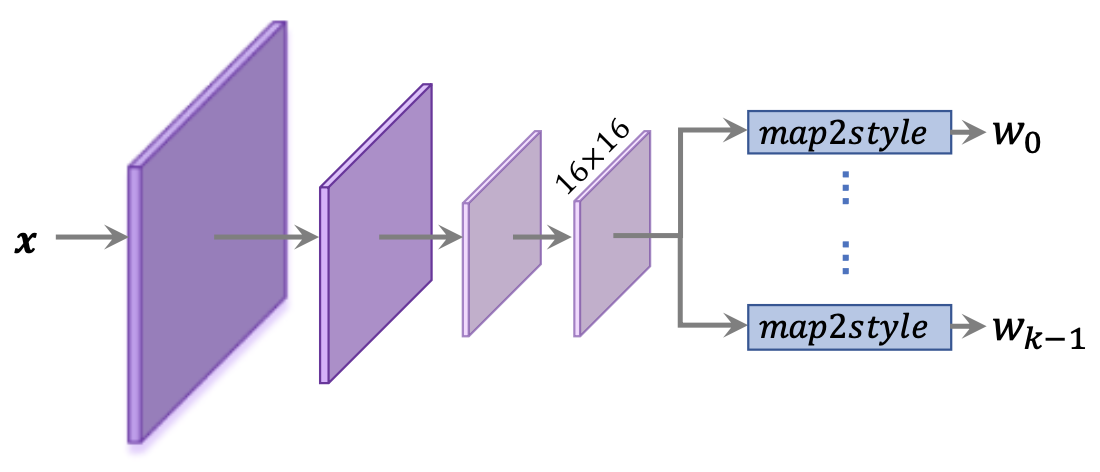
\includegraphics[scale=0.5]{figures/restyle-encoderArchitecture.png}
  \caption{Simplified ReStyle encoder architecture. Image taken from \cite{alaluf2021restyle}}
  \label{fig:ReStyle encoder architecture}
\end{figure}


 \subsubsection{ReStyle conclusion}
The ReStyle scheme has been shown to produce highly realistic results in a variety of experiments. It is capable of transforming the style of an image while preserving its content, which is a crucial property for style transfer algorithms. Additionally, the ReStyle algorithm is highly flexible, as it can be trained on different styles by using different pre-trained StyleGAN models. This allows for the creation of a large variety of style transfer models, each with a unique style.
